\documentclass[conference]{IEEEtran}
\usepackage[hidelinks]{hyperref}
\usepackage{graphicx}
\usepackage{amsmath}
\usepackage{adjustbox}
\usepackage{cite}
\usepackage{algorithm}

\usepackage{booktabs} % For better tables
\usepackage{microtype} % Better typography
\usepackage{xcolor}   % For colored text if needed
\usepackage{float}
\usepackage{listings}
\usepackage{algpseudocode}

\usepackage{tikz}
\usetikzlibrary{decorations.pathreplacing}
\usepackage[margin=1in]{geometry}

\definecolor{codegray}{rgb}{0.5,0.5,0.5}
\definecolor{backcolor}{rgb}{0.95,0.95,0.95}

% Draft TODO marker — remove before submission
\newcommand{\todo}[1]{\textcolor{red}{[TODO: #1]}}

\title{COALESCE: Coherence-Aware Perceptron Cache Replacement for Multithreaded Workloads}

\author{
  \IEEEauthorblockN{
    Harsh Raj\IEEEauthorrefmark{1}, \quad
    Bheemappa Halavar\IEEEauthorrefmark{1}
  }
  \\
  \vspace{-0.3cm}
  \IEEEauthorblockA{\IEEEauthorrefmark{1}Department of Computer Science and Engineering, IIIT Sri City, India \\
  }
  % TODO: confirm final author list and order with advisor before abstract registration
}

\begin{document}
\raggedbottom
\maketitle

\begin{abstract}
Learning-based last-level cache (LLC) replacement policies such as Hawkeye and Mockingjay define the state of the art, but they are evaluated almost exclusively on multi-programmed workloads---independent programs that share cache capacity without sharing data. We show that this evaluation regime hides a blind spot: under genuine multithreaded sharing, the state of the art collapses. Mockingjay, the strongest policy across one hundred multi-programmed mixes in its original evaluation, finishes last on three of the four multithreaded workloads in our study---up to 48\% behind SRRIP---and Hawkeye falls behind LRU on two of the four. We present COALESCE, a coherence-aware perceptron replacement policy whose features---program counter, MESI coherence state, and sharer count---are designed for coherent workloads. To evaluate it, we extend the ChampSim simulator, whose default per-CPU address spaces silently preclude all inter-core data sharing, with a shared-virtual-memory overlay that exposes coherence behaviour to the replacement policy. Across PARSEC and SPLASH-3 benchmarks at 4 to 16 cores, COALESCE achieves geometric-mean speedups of 9.7\% over LRU, 1.5\% over Hawkeye, and 13.9--22.5\% over Mockingjay, winning outright on canneal, the write-intensive irregular workload in our suite (5\% over Hawkeye and 30\% over Mockingjay at 8 cores). Feature ablation confirms that the sharer-count input contributes a stable 7\% under genuine cross-thread sharing. We characterise the workload properties---LLC pressure, access irregularity, and write fraction---that predict when coherence-aware replacement helps, and show that when they are absent, simple heuristics remain unbeaten.
\end{abstract}

\section{Introduction}

Modern multi-core processors share their last-level cache (LLC) among all cores, and the policy that decides which block to evict on a miss has a first-order effect on system throughput~\cite{hennessy2017quantitative}. A long line of work has progressively replaced static heuristics such as Least Recently Used (LRU) and Re-Reference Interval Prediction (RRIP)~\cite{jaleel2010rrip} with predictive, learning-based policies: SHiP learns reuse behaviour per program-counter signature~\cite{wu2011ship}, Hawkeye learns to imitate Belady's provably optimal MIN algorithm~\cite{belady1966study,jain2016hawkeye}, and Mockingjay refines this mimicry with fine-grained reuse-distance prediction, approaching the performance of MIN itself on its evaluation suite~\cite{shah2022mockingjay}.

These policies share an evaluation methodology as well as a lineage. They are validated on \emph{multi-programmed} workloads: collections of independent, single-threaded programs (typically drawn from SPEC CPU and GAP) co-scheduled on a multi-core simulator. In such workloads the cores \emph{compete} for LLC capacity but never \emph{share} data: no line is ever read by one core and written by another, no coherence invalidation ever removes a block, and the coherence state of every LLC line is trivial. Multithreaded applications---the workloads that shared LLCs were built for---behave fundamentally differently: threads communicate through shared lines, writes by one core invalidate copies held by others, and a block's coherence role carries information about its future reuse that no program-counter signature can see.

This paper asks a simple question: \emph{do state-of-the-art learned replacement policies, designed and tuned on multi-programmed workloads, transfer to genuine multithreaded sharing?} Answering it required removing an infrastructure obstacle. ChampSim~\cite{champsim2022}, the de-facto standard simulator of the cache-replacement community, assigns each simulated CPU a \emph{private} physical address space: two cores accessing the same virtual address receive different physical pages by construction. Every multi-core evaluation built on default ChampSim---including those of the policies above---is therefore multi-programmed by construction, even when the input traces come from a multithreaded program. We extend ChampSim's virtual memory subsystem with a \emph{shared-VMEM overlay} that maps identical virtual addresses from participating cores to the same physical page, restoring genuine inter-core sharing, coherence invalidations, and sharer tracking at the LLC (Section~\ref{sec:methodology}).

With this infrastructure we evaluate seven policies---LRU, SRRIP, DRRIP, SHiP, Hawkeye, Mockingjay, and our proposed COALESCE---on four multithreaded benchmarks from PARSEC~\cite{bienia2008parsec} and SPLASH-3~\cite{sakalis2016splash3} at 4, 8, and 16 cores. The results expose a clear blind spot. Mockingjay, the strongest policy in the multi-programmed world, finishes \emph{last} on three of the four workloads we test---trailing SRRIP by up to 48\%---and second-to-last among the baselines on the fourth. Hawkeye falls behind even LRU on two workloads. The implicit assumption that multi-programmed performance predicts multithreaded performance is false.

We then present COALESCE (Coherence-Observant Adaptive Learning for System-wide Cache Efficiency), a hashed-perceptron replacement policy~\cite{jimenez2001perceptron,jimenez2017multiperspective} whose feature set is chosen for coherent workloads: the program counter of the instruction that filled a block, the block's MESI coherence state, and its current sharer count. COALESCE wins outright on canneal, the most memory-intensive workload in our suite (5.0\% over Hawkeye and 30.5\% over Mockingjay at 8 cores; 47\% over LRU at 4 cores), and is the strongest learning-based policy on both workloads where capacity pressure and write traffic coincide (canneal and ocean). Across the full suite---including the workloads where it loses---COALESCE achieves geometric-mean speedups of 9.7\% over LRU and 1.5\% over Hawkeye at 4 cores.

This paper makes four contributions:
\begin{itemize}
  \item \textbf{A methodology contribution}: a shared-virtual-memory extension to ChampSim that enables, to our knowledge, the first evaluation of learned LLC replacement under genuine multithreaded data sharing (Section~\ref{sec:methodology}).
  \item \textbf{An evaluation finding}: state-of-the-art learned policies do not transfer to coherent workloads. Mockingjay places last on three of the four workloads (second-to-last among baselines on the fourth); Hawkeye loses to LRU on two (Section~\ref{sec:results}).
  \item \textbf{A policy}: COALESCE, a coherence-aware perceptron replacement policy that is the strongest learning-based policy on the capacity-pressured, write-active workloads in our suite, with a policy storage budget of ${\sim}44$\,KB for a 2\,MB LLC (Section~\ref{sec:design}).
  \item \textbf{A characterisation}: a feature ablation and workload analysis showing that the sharer-count feature contributes a stable 7\% exactly when cross-thread sharing is genuine, and identifying the three workload properties---LLC pressure, access irregularity, and write fraction---that predict when coherence-aware replacement helps (Sections~\ref{sec:ablation} and~\ref{sec:results}).
\end{itemize}

\section{Background and Motivation}
\label{sec:background}

\subsection{Learned cache replacement and its evaluation}

Belady's MIN algorithm~\cite{belady1966study} evicts the block whose next use is furthest in the future and is provably optimal, but requires knowledge of the future. Modern learned policies approximate it from history. SHiP~\cite{wu2011ship} associates re-reference behaviour with program-counter (PC) signatures. Hawkeye~\cite{jain2016hawkeye} reconstructs what MIN \emph{would have done} on a sampled history window (OPTgen) and trains a PC-indexed predictor to label load instructions cache-friendly or cache-averse. Mockingjay~\cite{shah2022mockingjay} replaces Hawkeye's binary labels with predicted reuse distances, tracked per PC in a sampled cache, and reports performance within 0.3\% of MIN's improvement bound on a single core. Glider~\cite{shi2019glider} and follow-on work apply offline deep learning to discover better features. Perceptron-based prediction in caches descends from Jiménez and Lin's branch predictor~\cite{jimenez2001perceptron}; multiperspective reuse prediction~\cite{jimenez2017multiperspective} hashes several program features into independent weight tables whose summed response drives a bypass/eviction decision.

All of these policies are evaluated on single-threaded traces (SPEC CPU 2006/2017, GAP, CVP) run either alone or as multi-programmed multi-core mixes. We are not aware of any published evaluation of these policies under multithreaded data sharing.

\subsection{What sharing changes}

In a multithreaded workload, the LLC is not merely contended capacity; it is the communication fabric between threads. This changes replacement in three ways. First, \emph{coherence state carries reuse information}: a block in MODIFIED state was recently written and---in producer-consumer and migratory sharing patterns---is disproportionately likely to be read soon by another core. Evicting it costs both the future reader and a writeback. Second, \emph{sharer count carries reuse information}: a line cached by several cores' private levels is part of the actively shared working set; evicting its LLC copy forces all sharers to refetch from memory. Third, \emph{invalidations break recency heuristics}: a write by one core removes copies from other cores' private caches, so LLC recency no longer reflects the line's system-wide liveness. None of these signals exist in a multi-programmed workload, where every line has exactly one ever-owner, no line is ever invalidated, and state never carries cross-core meaning.

\subsection{The simulator obstacle}
\label{sec:obstacle}

ChampSim~\cite{champsim2022} keys its virtual-to-physical mapping on the pair (CPU, virtual address): two cores touching the same virtual address are assigned \emph{different} physical pages. This is convenient for multi-programmed studies---identical SPEC traces can be replicated across cores without aliasing---but it makes genuine sharing impossible: even traces captured from one multithreaded process are silently privatised, every sharer count is 1, and the number of coherence invalidations at the LLC is exactly zero on every run. We verified this empirically on our workloads before this study; it motivates the overlay described next.

\section{The COALESCE Policy}
\label{sec:design}

COALESCE is a hashed-perceptron replacement policy in the lineage of multiperspective reuse prediction~\cite{jimenez2017multiperspective}, with a feature set chosen for coherent workloads. It comprises two perceptron weight tables, a per-sampled-set ghost filter for eviction feedback, and an explicit coherence bias; Table~\ref{tab:storage} itemises the structures.

\subsection{Prediction structures}

Two independent weight tables of 2{,}048 8-bit saturating entries each ($[-128, +127]$) are indexed by orthogonal hashes of the candidate block's metadata:
\begin{equation}
h_0 = \mathrm{hash}\big(\mathrm{PC} \oplus \mathrm{0x9e3779b9},\ \mathrm{state}\big) \bmod 2048,
\end{equation}
\begin{equation}
h_1 = \mathrm{hash}\big(\mathrm{PC} \oplus \mathrm{0x85ebca6b},\ \mathrm{sharers}\big) \bmod 2048,
\end{equation}
where PC is the program counter of the instruction that most recently filled or touched the block, \emph{state} is the block's MESI state, and \emph{sharers} is the population count of its sharer mask. The raw vote for a block is the sum $w_0[h_0] + w_1[h_1]$: large positive votes mean ``keep'', large negative votes mean ``safe to evict''.

\subsection{Coherence bias}

On top of the learned vote, COALESCE applies an explicit coherence bias, but only to blocks the perceptron already considers worth keeping (raw vote $> 0$):
\begin{equation}
\mathrm{vote} \mathrel{+}=
\begin{cases}
+40 & \text{if state} = \text{MODIFIED},\\
+20 \times \mathrm{sharers} & \text{if sharers} \geq 2.
\end{cases}
\label{eq:bias}
\end{equation}
The gating prevents the bias from rescuing blocks the perceptron has confidently learned are dead. The victim is the way with the \emph{lowest} final vote (Algorithm~\ref{alg:victim}).

\begin{algorithm}[H]
\small
\caption{Victim Selection in COALESCE}
\label{alg:victim}
\begin{algorithmic}[1]
\Procedure{FindVictim}{$set$}
    \State $victim \gets 0$, $minVote \gets +\infty$
    \For{$way \gets 0$ to $NUM\_WAY - 1$}
        \If{$\neg\, block[way].valid$} \Return $way$ \EndIf
        \State $v \gets w_0[h_0(\mathrm{PC}, \mathrm{state})] + w_1[h_1(\mathrm{PC}, \mathrm{sharers})]$
        \If{$v > 0$}
            \If{$state = \mathrm{MODIFIED}$} $v \gets v + 40$ \EndIf
            \If{$sharers \geq 2$} $v \gets v + 20 \times sharers$ \EndIf
        \EndIf
        \If{$v < minVote$} $minVote \gets v$;\ $victim \gets way$ \EndIf
    \EndFor
    \If{$set$ is sampled} record victim in ghost filter \EndIf
    \State \Return $victim$
\EndProcedure
\end{algorithmic}
\end{algorithm}

\subsection{Training and the ghost-rescue mechanism}

Training is confined to sampled sets (every 32nd set, 3.125\% of the cache) to bound metadata cost, following the set-sampling tradition of DRRIP and Hawkeye~\cite{jaleel2010rrip,jain2016hawkeye}. On a hit in a sampled set, the weights at $h_0$ and $h_1$ are incremented (reward) when the current vote is mispredicting or has magnitude below a confidence threshold $\theta = 35$, a training rule adapted from perceptron branch prediction~\cite{jimenez2001perceptron}.

Misses train through a \emph{ghost rescue} path. Each sampled set maintains a 1{,}024-bit Bloom filter (3 hash functions, reset every 150 insertions) and a 128-entry direct-mapped ghost table of recently evicted blocks; each 32-bit ghost entry packs a 12-bit PC signature, 14-bit partial tag, 3-bit sharer count, 2-bit MESI state, and a valid bit. When a miss matches a ghost entry---evidence that the policy evicted a block that was still live---the corresponding weights receive a boosted reward ($5\times$ repetition), rapidly rehabilitating the mispredicted context.

\subsection{Storage cost}
\label{sec:storage}

Table~\ref{tab:storage} itemises the policy storage. MESI state and the sharer mask are maintained by the coherence substrate of any real multi-core (directory or snoop filter) and are read, not duplicated, by COALESCE; we therefore count only policy-private structures, as is conventional~\cite{jain2016hawkeye,shah2022mockingjay}. The total is ${\sim}44$\,KB for a 2\,MB LLC ($\sim$2.1\% of the data array), comparable to the budgets of Hawkeye and Mockingjay under the cache-replacement-championship convention.

\begin{table}[htbp]
    \centering
    \renewcommand{\arraystretch}{1.2}
    \caption{COALESCE policy storage for a 2\,MB, 2048-set LLC}
    \label{tab:storage}
    \resizebox{0.95\linewidth}{!}{%
    \begin{tabular}{lll}
        \toprule
        \textbf{Structure} & \textbf{Sizing} & \textbf{Cost} \\
        \midrule
        Perceptron tables & $2 \times 2048 \times 8$\,bits & 4\,KB \\
        Bloom filters & $64$ sampled sets $\times\ 1024$\,bits & 8\,KB \\
        Ghost tables & $64 \times 128$ entries $\times\ 32$\,bits & 32\,KB \\
        \midrule
        \textbf{Total} & & \textbf{44\,KB} \\
        \bottomrule
    \end{tabular}
    }
\end{table}

\section{Experimental Methodology}
\label{sec:methodology}

\subsection{Shared-VMEM overlay}

We extend ChampSim's \texttt{VirtualMemory} with a configurable set of \emph{sharing CPUs}. For CPUs in this set, the virtual-to-physical mapping is keyed on the virtual address alone, so identical virtual addresses from different cores resolve to the same physical page---restoring the semantics of threads within one process. Fills that hit a page mapped by another core are tracked (\emph{aliased fills}), the LLC maintains a per-line sharer mask and MESI state, and writes to lines with remote sharers generate coherence invalidations, all of which are exposed to the replacement policy and reported in statistics. The overlay is ${\sim}100$ lines of simulator change and is independent of any policy; we will release it with the paper. All experiments in this paper, for all policies, run under the overlay; Section~\ref{sec:threats} discusses the default-VMEM (private) configuration.

\subsection{System configuration}

Table~\ref{tab:simconfig} lists the simulated system. The LLC is shared by all cores; private L1/L2 caches and TLBs use ChampSim defaults. No prefetcher is used at any level, isolating the replacement policy's effect, consistent with the no-prefetcher configurations of prior replacement studies~\cite{jain2016hawkeye,shah2022mockingjay}.

\begin{table}[htbp]
    \centering
    \caption{Simulation Configuration}
    \label{tab:simconfig}
    \resizebox{0.95\linewidth}{!}{%
    \begin{tabular}{ll}
        \toprule
        \textbf{Parameter} & \textbf{Value} \\
        \midrule
        Cores & 4, 8, 16 (out-of-order, ChampSim default core) \\
        Shared LLC & 2\,MB, 2048 sets $\times$ 16 ways, 64\,B lines \\
        Private L1I/L1D/L2 & ChampSim defaults per core \\
        DRAM & DDR4-3200, $t_{RP}=t_{RCD}=t_{CAS}=24$ \\
        Virtual memory & shared-VMEM overlay across all cores \\
        Prefetcher & none \\
        Warmup / simulation & 50\,M / 100\,M instructions per core \\
        Replacement policies & LRU, SRRIP, DRRIP, SHiP, Hawkeye, \\
        & Mockingjay, COALESCE (+ ablation) \\
        \bottomrule
    \end{tabular}
    }
\end{table}

\subsection{Workloads}

We use four multithreaded benchmarks chosen to span distinct LLC behaviours (Table~\ref{tab:workloads}): \texttt{canneal} (PARSEC; simulated-annealing netlist routing---pointer-chasing, write-heavy, far exceeding LLC capacity), \texttt{ocean\_cp} (SPLASH-3; multigrid PDE solver---regular grid sweeps, mixed read/write, capacity-pressured), \texttt{fluidanimate} (PARSEC; particle simulation whose LLC traffic is 100\% reads), and \texttt{barnes} (SPLASH-3; N-body octree whose working set at the standard $n{=}16384$ input fits within the LLC). Traces are captured per thread with a Pin-based tracer~\cite{luk2005pin} and replayed with one thread per core; at 8 and 16 cores, thread traces are replicated in the same pattern for all policies, so all comparisons are like-for-like. Within each benchmark and core count, every policy executes an identical instruction volume.

\begin{table}[htbp]
    \centering
    \renewcommand{\arraystretch}{1.2}
    \caption{Workload characterisation at the shared LLC (8 cores)}
    \label{tab:workloads}
    \resizebox{\linewidth}{!}{%
    \begin{tabular}{lllll}
        \toprule
        \textbf{Property} & \texttt{canneal} & \texttt{ocean} & \texttt{fluidanim.} & \texttt{barnes} \\
        \midrule
        Access pattern & irregular & regular & regular & irregular \\
        LLC write fraction & ${\sim}89\%$ & ${\sim}40\%$ & $0\%$ & mixed \\
        Working set vs.\ LLC & $\gg$ & $\gg$ & $>$ & $<$ \\
        LLC invalidations & 6.9\,M & 0.72\,M & 0 & 0.03\,M \\
        Lines with $\geq$2 sharers & 25.6\% & high & ${\sim}0$ & low \\
        \bottomrule
    \end{tabular}
    }
\end{table}

\subsection{Baselines and metrics}

LRU, SRRIP, DRRIP, and SHiP use ChampSim's standard implementations. We implemented Hawkeye (OPTgen with sampled history plus a PC-indexed predictor)~\cite{jain2016hawkeye} and Mockingjay (sampled reuse-distance prediction with estimated time remaining)~\cite{shah2022mockingjay} as ChampSim modules following the original papers. Our primary metric is \emph{total execution cycles}: the cycle count at which the last core completes its 100\,M-instruction region (lower is better). Because multithreaded cores interact through the shared LLC, per-core IPC is reported only for bottleneck analysis. Speedups are reported as cycle-count ratios and summarised by geometric mean.

\section{Results}
\label{sec:results}

\subsection{canneal: where coherence-aware learning wins}
\label{sec:canneal}

Figure~\ref{fig:canneal} and Table~\ref{tab:canneal} report total cycles on canneal. At 4 cores COALESCE finishes in 267.3\,M cycles---7.3\% ahead of Hawkeye, the best baseline, and 47.1\% ahead of LRU. At 8 cores COALESCE remains first at 301.9\,M cycles, 0.4\% ahead of SRRIP, 4.8\% ahead of SHiP, 5.0\% ahead of Hawkeye, and 30\% ahead of both LRU and Mockingjay.

canneal is precisely the workload class COALESCE targets: its LLC traffic is ${\sim}89\%$ writes (RFO + writeback), its pointer-chasing access pattern defeats recency and RRIP-style position heuristics, and its working set vastly exceeds the 2\,MB LLC, so every eviction decision matters. Under the shared overlay its coherence machinery is highly active (6.9\,M invalidations; one quarter of evicted lines have two or more sharers at 8 cores), giving the MESI and sharer features genuine signal.

\begin{table}[htbp]
    \centering
    \renewcommand{\arraystretch}{1.15}
    \caption{canneal total cycles (lower is better)}
    \label{tab:canneal}
    \resizebox{0.9\linewidth}{!}{%
    \begin{tabular}{lrrrr}
        \toprule
        \textbf{Policy} & \textbf{4-core} & vs.\ C. & \textbf{8-core} & vs.\ C. \\
        \midrule
        \textbf{COALESCE} & \textbf{267{,}251{,}645} & --- & \textbf{301{,}945{,}789} & --- \\
        Hawkeye & 286{,}865{,}528 & $+7.3\%$ & 317{,}172{,}523 & $+5.0\%$ \\
        SRRIP & 287{,}031{,}501 & $+7.4\%$ & 303{,}011{,}899 & $+0.4\%$ \\
        SHiP & 288{,}163{,}881 & $+7.8\%$ & 316{,}393{,}994 & $+4.8\%$ \\
        DRRIP & 294{,}947{,}400 & $+10.4\%$ & 325{,}848{,}199 & $+7.9\%$ \\
        Mockingjay & 311{,}277{,}369 & $+16.5\%$ & 393{,}934{,}080 & $+30.5\%$ \\
        LRU & 392{,}999{,}637 & $+47.1\%$ & 392{,}564{,}736 & $+30.0\%$ \\
        \bottomrule
    \end{tabular}
    }
\end{table}

\begin{figure}[H]
    \centering
    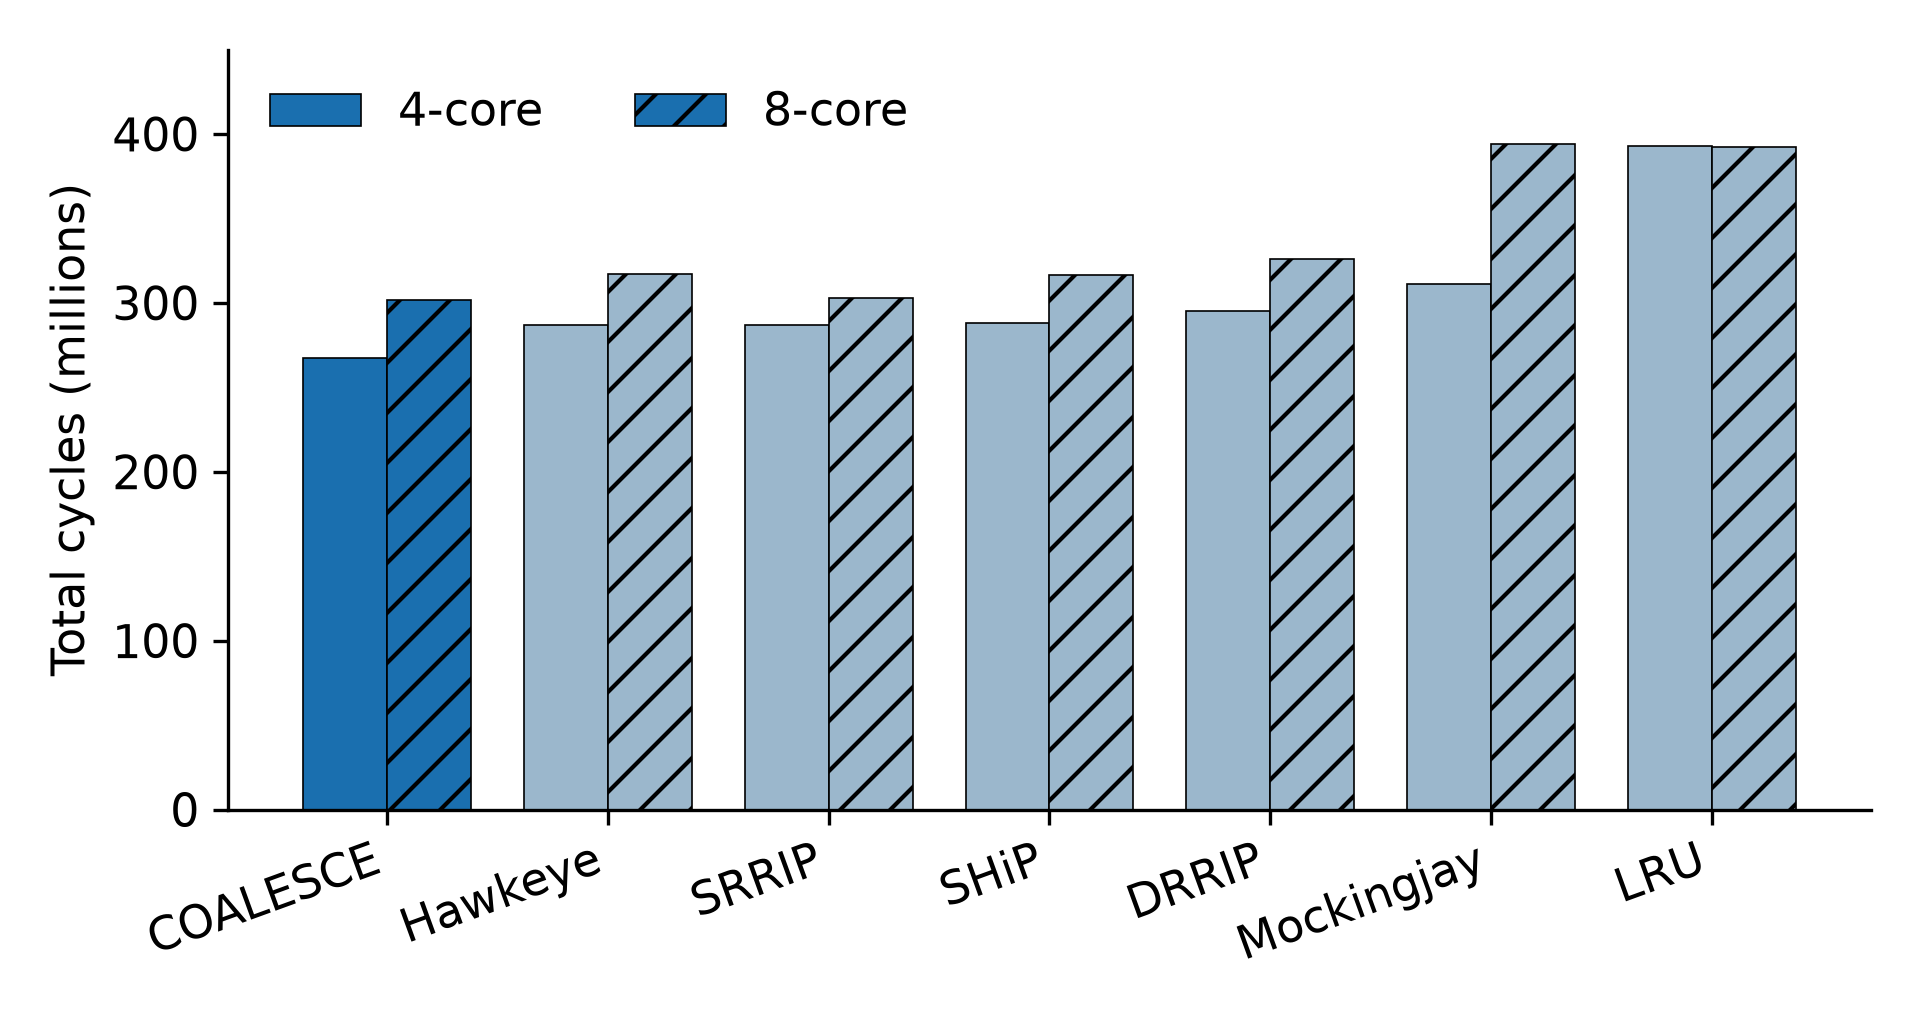
\includegraphics[width=0.95\linewidth]{fig_canneal.png}
    \caption{canneal total execution cycles at 4 and 8 cores (lower is better). COALESCE is first at both scales.}
    \label{fig:canneal}
\end{figure}

At 16 cores under the overlay, COALESCE completes the same per-core work in 348.2\,M cycles, with bottleneck-core IPC declining only modestly (0.374 at 4 cores, 0.332 at 8, 0.294 at 16) as per-core effective LLC capacity shrinks by $4\times$ (Figure~\ref{fig:scaling}). Per-policy comparisons at 16 cores were not run due to compute budget; the 8-core comparison is representative.

\begin{figure}[H]
    \centering
    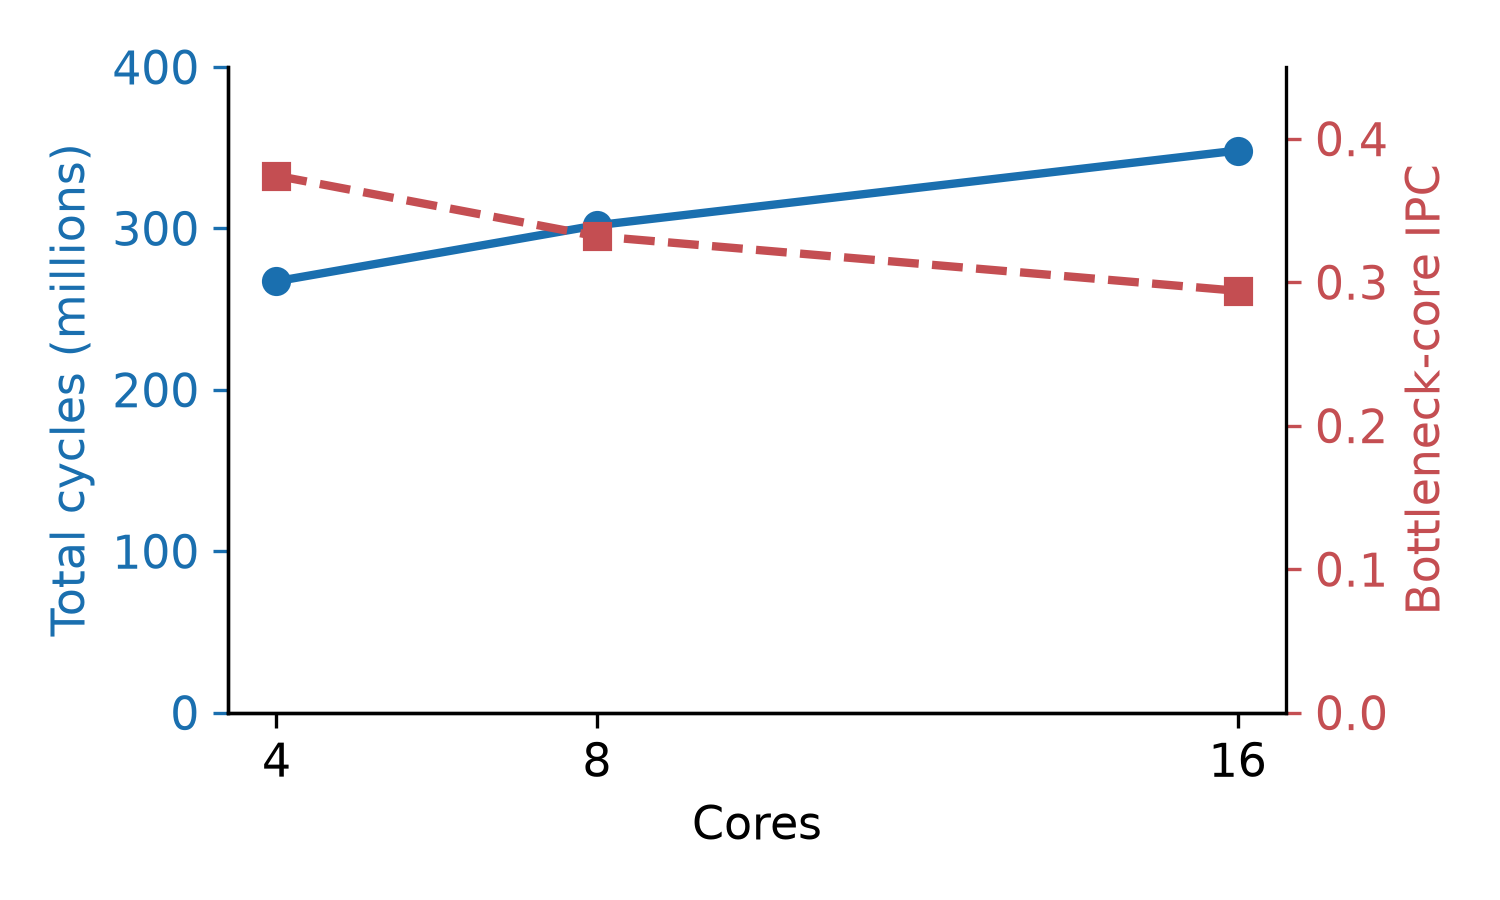
\includegraphics[width=0.95\linewidth]{fig_scaling.png}
    \caption{COALESCE scaling on canneal: total cycles and bottleneck-core IPC at 4, 8, and 16 cores.}
    \label{fig:scaling}
\end{figure}

\subsection{ocean: regular access favours RRIP heuristics}
\label{sec:ocean}

On ocean (Table~\ref{tab:ocean}) the RRIP family wins: SHiP, SRRIP, and DRRIP finish within 0.4\% of one another, with COALESCE fourth, 3.6\% behind at 4 cores and 2.9\% behind at 8 cores. The mechanism is no mystery: ocean's multigrid sweeps are regular and stride-predictable---exactly the re-reference geometry that RRIP's insertion heuristics were designed around~\cite{jaleel2010rrip}---and although its coherence traffic is substantial ($6\times$ canneal's invalidation rate per LLC access), regularity, not sharing, dominates the eviction decision.

The notable result is the fate of the \emph{learning} policies. COALESCE is the best of them at both scales: it beats Hawkeye by 3.5--4.3\% and LRU by ${\sim}3\%$, while Mockingjay degrades sharply, to 48\% behind SRRIP (Section~\ref{sec:mockingjay}). On coherent workloads, learning does not automatically lose to heuristics---but learning \emph{tuned on the wrong distribution} does.

\begin{table}[htbp]
    \centering
    \renewcommand{\arraystretch}{1.15}
    \caption{ocean total cycles (lower is better)}
    \label{tab:ocean}
    \resizebox{0.9\linewidth}{!}{%
    \begin{tabular}{lrrrr}
        \toprule
        \textbf{Policy} & \textbf{4-core} & vs.\ best & \textbf{8-core} & vs.\ best \\
        \midrule
        SHiP & \textbf{549{,}605{,}858} & --- & 550{,}732{,}443 & $+0.01\%$ \\
        SRRIP & 550{,}297{,}702 & $+0.1\%$ & \textbf{550{,}675{,}830} & --- \\
        DRRIP & 551{,}685{,}991 & $+0.4\%$ & 551{,}564{,}285 & $+0.2\%$ \\
        \textbf{COALESCE} & 569{,}457{,}207 & $+3.6\%$ & 566{,}374{,}131 & $+2.9\%$ \\
        LRU & 587{,}215{,}973 & $+6.8\%$ & 584{,}499{,}393 & $+6.1\%$ \\
        Hawkeye & 589{,}923{,}943 & $+7.3\%$ & 591{,}008{,}754 & $+7.3\%$ \\
        Mockingjay & 813{,}767{,}568 & $+48.1\%$ & 814{,}696{,}310 & $+47.9\%$ \\
        \bottomrule
    \end{tabular}
    }
\end{table}

\subsection{fluidanimate and barnes: the boundaries}
\label{sec:boundaries}

The remaining two workloads delimit where coherence-aware replacement cannot help, and we report them as such.

\textbf{fluidanimate}'s LLC traffic is 100\% loads: lines are never written at the LLC, MESI state never leaves EXCLUSIVE, invalidations are exactly zero, and both coherence features of COALESCE are structurally unable to fire. The total policy spread is only ${\sim}5\%$, and COALESCE is last within it (4.9--5.0\% behind DRRIP at both 4 and 8 cores)---paying its prediction overhead for features that carry no signal on this workload. The consistency of this deficit across core counts confirms it is mechanism, not noise.

\textbf{barnes} at the standard $n{=}16384$ input has a working set ($\sim$1.6\,MB) that fits within the 2\,MB LLC: the LLC observes only ${\sim}500$\,K accesses and evictions are rare, so replacement choices barely matter. All eight policies finish within 3.8\% of one another and LRU---the cheapest---wins; COALESCE trails it by 2.5\%. Low LLC pressure is the third boundary condition: when nothing is evicted, no replacement policy can earn its overhead.

\subsection{The multi-programmed state of the art does not transfer}
\label{sec:mockingjay}

Across all four workloads a consistent pattern emerges for the strongest multi-programmed policies (Figure~\ref{fig:geomean}). Mockingjay---which improves on LRU by 15.2\% averaged over one hundred multi-programmed mixes in its original evaluation~\cite{shah2022mockingjay}---finishes \emph{last on three of the four workloads in this study} and second-to-last among the baselines on the fourth: 30.5\% behind COALESCE on canneal at 8 cores, 48\% behind SRRIP on ocean at both scales, and behind LRU on fluidanimate and barnes. Hawkeye fares better but still loses to LRU on ocean and barnes. We attribute this to distribution shift: Mockingjay's reuse-distance predictor is trained online from PC-indexed samples that, under multithreaded sharing, conflate accesses from different cores to the same lines; invalidations remove blocks at times its estimated-time-remaining model cannot anticipate. A policy that approaches MIN on the distribution it was designed for can sit below LRU outside it. We believe this is the paper's most consequential observation for the field: \emph{evaluation methodology, not predictor capacity, is the current bottleneck for learned replacement on multithreaded workloads.}

\subsection{Suite-wide summary}

Figure~\ref{fig:geomean} reports geometric-mean speedups of COALESCE over each baseline across the full suite, losses included. COALESCE achieves $+9.7\%$ over LRU, $+1.5\%$ over Hawkeye, and $+13.9\%$ over Mockingjay at 4 cores (4 benchmarks), and $+9.2\%$, $+1.5\%$, and $+22.5\%$ respectively at 8 cores (3 benchmarks; barnes was run at 4 cores). Against the RRIP family COALESCE is between $+0.2\%$ and $-2.4\%$---a fair summary of a policy that wins decisively inside its target class and concedes modest ground outside it. Among learning-based policies, COALESCE attains the highest geomean over LRU at both scales ($+9.7\%$/$+9.2\%$, against Hawkeye's $+8.1\%$/$+7.5\%$; Mockingjay's is net negative at $-3.7\%$/$-10.9\%$).

\begin{figure}[H]
    \centering
    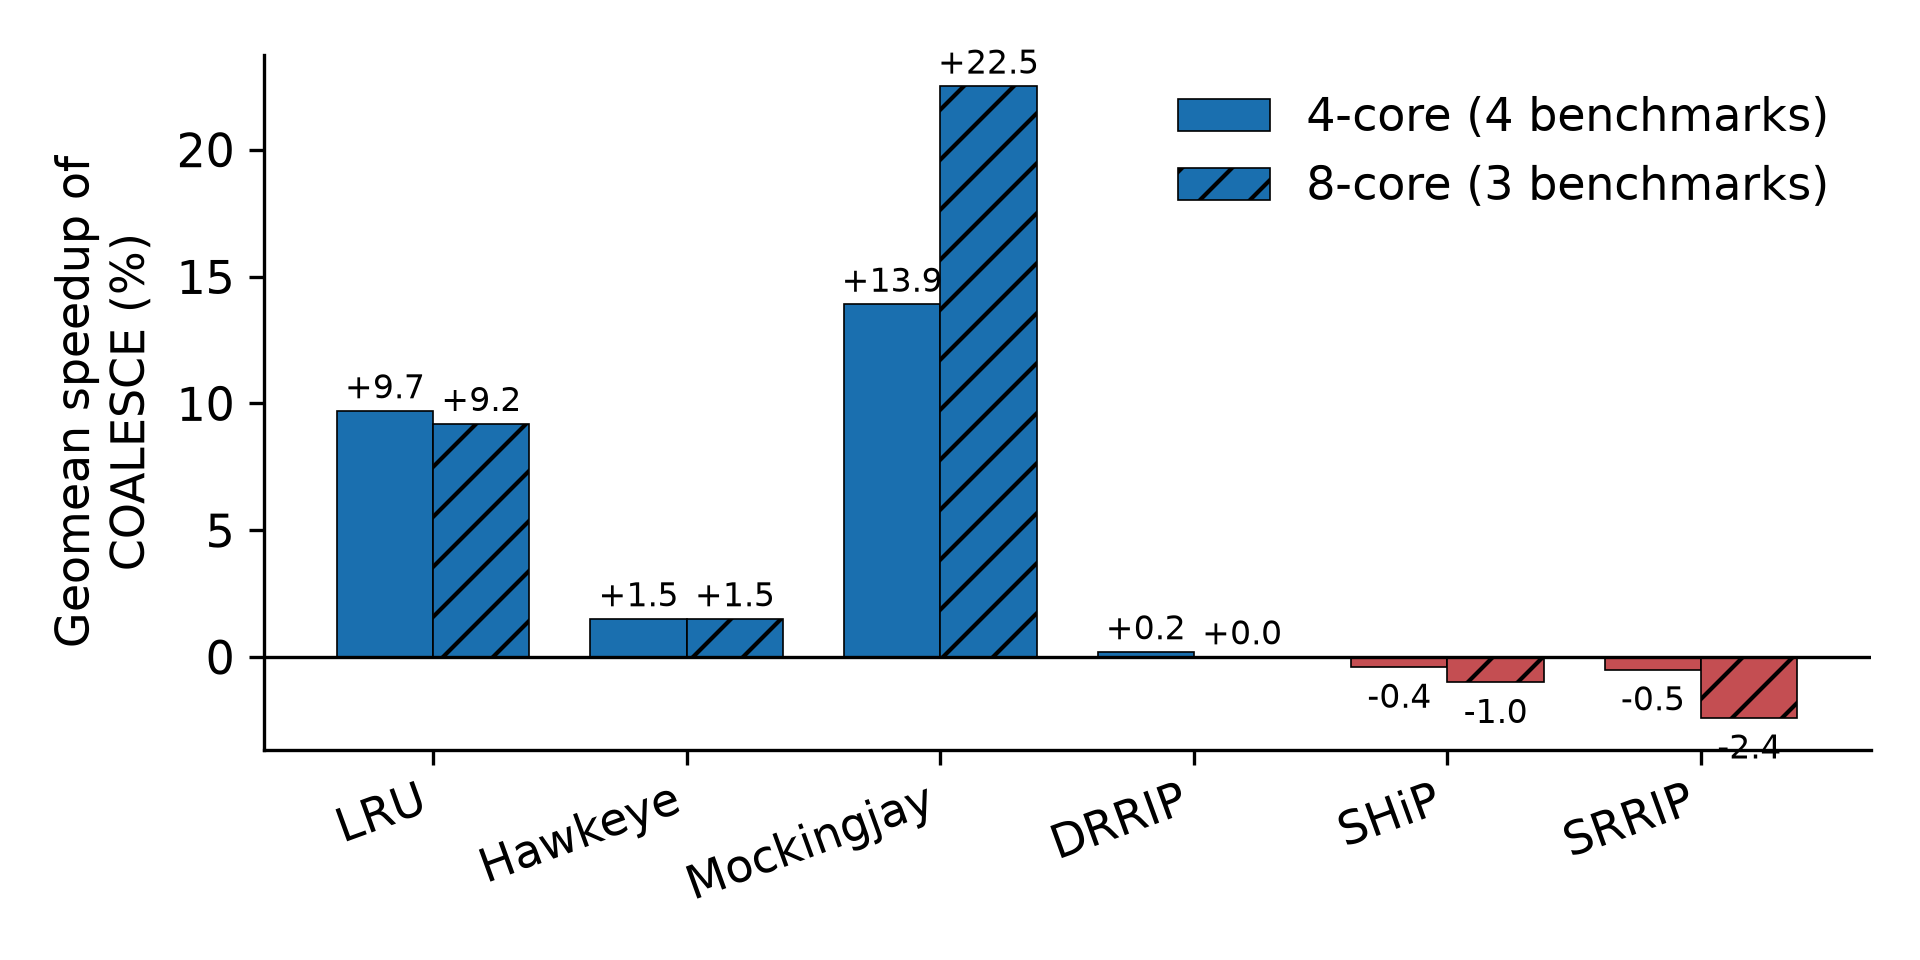
\includegraphics[width=0.95\linewidth]{fig_geomean.png}
    \caption{Geometric-mean speedup of COALESCE over each baseline across all workloads (losses included), at 4 cores (4 benchmarks) and 8 cores (3 benchmarks).}
    \label{fig:geomean}
\end{figure}

\subsection{Run-to-run variance}

\todo{Insert seed-variance numbers when the 3-seed runs land: across three VMEM randomisation seeds on a fixed 8-core canneal configuration, report per-policy max-cycle ranges and confirm rank stability. Note for drafting: the seed study uses its own fixed trace mix and is reported as a separate variance experiment, not as error bars on Table~\ref{tab:canneal}.}

\section{Feature Ablation: When Does the Sharer Count Matter?}
\label{sec:ablation}

Reviewers of any multi-feature policy should ask whether each feature earns its storage. We ablate COALESCE's sharer-count axis: the ablated variant (\emph{no-sharer}) replaces $h_1$'s sharer input with a second PC-only hash (a distinct mixing constant, after~\cite{jimenez2017multiperspective}) and removes the $+20\times$sharers bias, leaving the MESI axis and all other machinery intact. Figure~\ref{fig:ablation} and Table~\ref{tab:ablation} compare the two on every workload.

\begin{table}[htbp]
    \centering
    \renewcommand{\arraystretch}{1.15}
    \caption{Ablation: full COALESCE vs.\ no-sharer variant (total cycles; $\Delta>0$ means the sharer feature helps)}
    \label{tab:ablation}
    \resizebox{\linewidth}{!}{%
    \begin{tabular}{lrrr}
        \toprule
        \textbf{Workload} & \textbf{COALESCE} & \textbf{no-sharer} & $\Delta$ \\
        \midrule
        canneal 4-core & 267{,}251{,}645 & 267{,}247{,}657 & $-0.002\%$ \\
        canneal 8-core & 301{,}945{,}789 & 300{,}714{,}619 & $-0.41\%$ \\
        ocean 4-core & 569{,}457{,}207 & 611{,}083{,}533 & $\mathbf{+7.3\%}$ \\
        ocean 8-core & 566{,}374{,}131 & 607{,}309{,}316 & $\mathbf{+7.2\%}$ \\
        barnes 4-core & 160{,}448{,}239 & 160{,}656{,}244 & $+0.1\%$ \\
        \bottomrule
    \end{tabular}
    }
\end{table}

\begin{figure}[H]
    \centering
    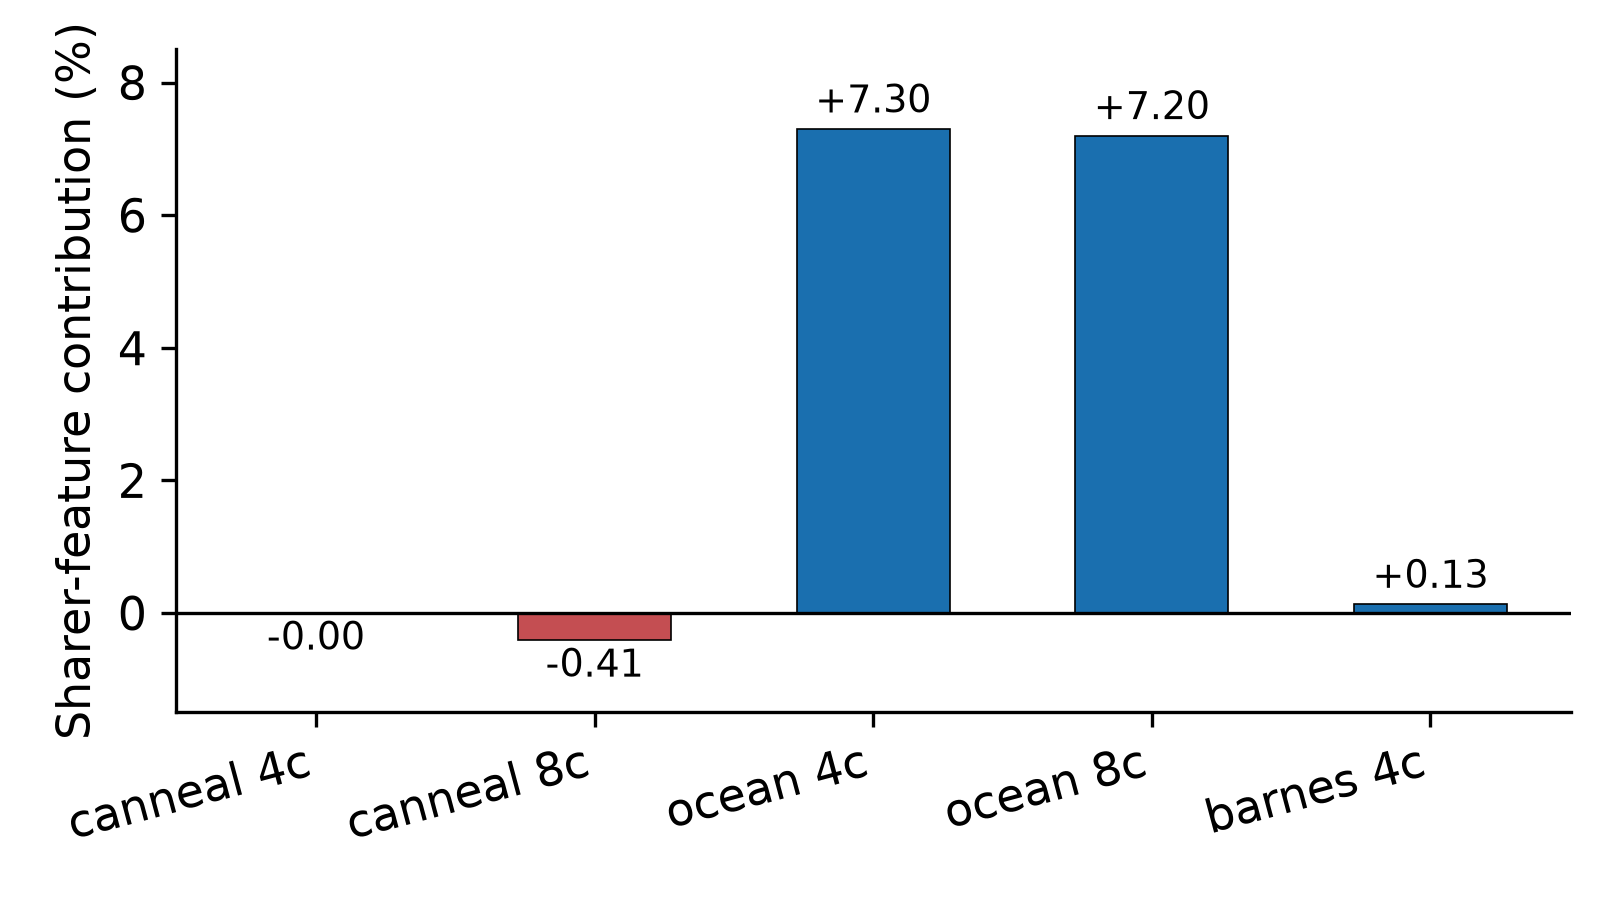
\includegraphics[width=0.95\linewidth]{fig_ablation.png}
    \caption{Contribution of the sharer-count feature (positive = full COALESCE faster than the no-sharer ablation).}
    \label{fig:ablation}
\end{figure}

The result is a clean dichotomy. On canneal, whose cross-thread sharing is shallow (only 1.45\% of evicted lines have $\geq 2$ sharers at 4 cores), the sharer feature is inert at 4 cores and marginally harmful at 8 cores ($-0.41\%$), where the $+20\times$sharers bias occasionally fires on noise. On ocean, whose grid-boundary exchange produces genuine multi-sharer lines, the feature contributes a stable $+7.2$--$7.3\%$ at both scales---without it, COALESCE would fall from 3\% to 11\% behind SRRIP. The feature is not dead weight and not universally useful: \emph{it activates exactly when the workload actually shares}. This motivates keeping the full feature set as the default design and explains both results in Section~\ref{sec:results} mechanistically: the MESI axis carries canneal; the sharer axis defends ocean.

\section{Threats to Validity}
\label{sec:threats}

\textbf{Workload coverage.} Four multithreaded benchmarks is small compared to the 30--100 single-threaded traces of multi-programmed studies~\cite{shi2019glider,shah2022mockingjay}; each of our runs, however, is a full multi-core coherent simulation rather than a replicated single-core trace, and the four were chosen to span the characterisation space of Table~\ref{tab:workloads} (write-heavy irregular, write-mixed regular, read-only, and low-pressure). Coherence-stress workloads (e.g., GAP graph kernels run multithreaded, SPLASH-3 water) are future work.

\textbf{Simulation regime.} All results use our shared-VMEM overlay. Under default ChampSim (private per-core address spaces) we observe larger absolute gaps in COALESCE's favour---e.g., $+33\%$ over SRRIP on 8-core canneal---but we regard that regime as an artefact of the simulator's memory model rather than a property of any policy, and report only the shared regime. We model MESI state and invalidation at the LLC; a full directory protocol with private-cache back-invalidation timing may shift constants but not, we believe, the structural findings.

\textbf{Input scale.} barnes uses the standard $n{=}16384$ input, whose working set fits in the LLC; larger inputs would pressure the cache but were precluded by a static array limit in the reference binary. We report barnes as the low-pressure boundary case it is.

\textbf{Baseline fidelity.} Hawkeye and Mockingjay are our reimplementations from the original papers; both reproduce their expected behaviour on capacity-contended workloads (e.g., Hawkeye is the best baseline on 4-core canneal). Their degradation under sharing is consistent across all workloads and scales, which argues against an implementation artefact, but independent replication would strengthen this finding.

\textbf{Single LLC size.} All experiments use a 2\,MB shared LLC. The characterisation predicts that growing the LLC moves workloads toward the barnes (low-pressure) corner and shrinking it deepens capacity effects; a size sweep is left to future work.

\section{Related Work}
\label{sec:related}

\textbf{Heuristic replacement.} LRU and its approximations dominate practice; RRIP~\cite{jaleel2010rrip} re-references blocks by predicted interval and remains, with SHiP's PC-signature insertion~\cite{wu2011ship}, the strongest cheap baseline---a position our ocean results reaffirm under sharing.

\textbf{Learned replacement.} Hawkeye~\cite{jain2016hawkeye} casts replacement as supervised imitation of Belady's MIN~\cite{belady1966study}; Mockingjay~\cite{shah2022mockingjay} sharpens the target from binary labels to reuse distances; Glider~\cite{shi2019glider} distils offline deep models into deployable predictors; multiperspective reuse prediction~\cite{jimenez2017multiperspective} and perceptron-based reuse prediction bring the hashed-perceptron idiom~\cite{jimenez2001perceptron} to caches, which COALESCE adopts. Cost-conscious learned policies have also been designed with reinforcement learning~\cite{sethumurugan2021designing,souza2024rl} and concurrency-aware perceptrons for GPU-class miss-cost prediction~\cite{wu2025camp}. All of these evaluate on single-threaded or multi-programmed workloads; none observe coherence state. To our knowledge COALESCE is the first replacement policy to use MESI state and sharer count as learned features, and this paper is the first head-to-head evaluation of learned replacement under genuine multithreaded sharing.

\textbf{Coherence-aware cache management.} Coherence information has been exploited for purposes other than replacement: deactivating coherence for private blocks to shrink directories~\cite{cuesta2011coherence}, OS-assisted classification for block placement and replication in NUCA caches~\cite{hardavellas2009rnuca}, and measurement studies quantifying coherence's performance impact on real multiprocessors~\cite{molka2009memory}. These works treat coherence metadata as a management signal but leave the replacement policy untouched; COALESCE closes that gap.

\textbf{Multithreaded benchmarking.} PARSEC~\cite{bienia2008parsec} and SPLASH-3~\cite{sakalis2016splash3} (a data-race-free revision of SPLASH-2~\cite{woo1995splash2}) are the standard shared-memory suites; our Pin-based~\cite{luk2005pin} per-thread tracing and shared-VMEM replay bring them to ChampSim-class replacement studies for the first time.

\section{Conclusion}

We presented the first evaluation of learned LLC replacement under genuine multithreaded data sharing, enabled by a shared-virtual-memory overlay for ChampSim, and a new coherence-aware perceptron policy, COALESCE, designed for that regime. The evaluation yields three durable findings. First, the multi-programmed state of the art does not transfer: Mockingjay places last on three of the four workloads tested and Hawkeye falls behind LRU on half of them---evidence that evaluation methodology, not model capacity, currently limits learned replacement. Second, coherence features earn their cost exactly where coherence is real: COALESCE wins outright on the write-heavy irregular canneal (5\% over Hawkeye, 30\% over Mockingjay at 8 cores) and its sharer-count feature contributes a reproducible 7\% on genuinely-shared workloads while remaining inert elsewhere. Third, the boundaries are predictable: regular access patterns favour RRIP heuristics, read-only LLC traffic disables coherence features, and low LLC pressure makes all policies equivalent---a three-axis characterisation that practitioners can apply before deploying any learned policy.

Future work follows directly: multithreaded GAP and coherence-stress SPLASH workloads to populate the high-sharing corner of the characterisation; LLC size sweeps; a directory-accurate coherence model; and, most promisingly, a policy designed \emph{from} the characterisation---one that learns online which of its feature axes the running workload activates, rather than weighting them statically.

\begin{thebibliography}{20}

\bibitem{belady1966study}
L. A. Belady,
``A study of replacement algorithms for a virtual-storage computer,''
\textit{IBM Systems Journal}, vol. 5, no. 2, pp. 78--101, 1966,
doi: \href{https://doi.org/10.1147/sj.52.0078}{10.1147/sj.52.0078}.

\bibitem{jaleel2010rrip}
A. Jaleel, K. B. Theobald, S. C. Steely Jr., and J. Emer,
``High performance cache replacement using re-reference interval prediction (RRIP),''
in \textit{Proc. 37th Int. Symp. Computer Architecture (ISCA)},
Saint-Malo, France, 2010, pp. 60--71,
doi: \href{https://doi.org/10.1145/1815961.1815971}{10.1145/1815961.1815971}.

\bibitem{wu2011ship}
C.-J. Wu, A. Jaleel, W. Hasenplaugh, M. Martonosi, S. C. Steely Jr., and J. Emer,
``SHiP: Signature-based hit predictor for high performance caching,''
in \textit{Proc. 44th IEEE/ACM Int. Symp. Microarchitecture (MICRO)},
Porto Alegre, Brazil, 2011, pp. 430--441,
doi: \href{https://doi.org/10.1145/2155620.2155671}{10.1145/2155620.2155671}.

\bibitem{jain2016hawkeye}
A. Jain and C. Lin,
``Back to the future: Leveraging Belady's algorithm for improved cache replacement,''
in \textit{Proc. 43rd Int. Symp. Computer Architecture (ISCA)},
Seoul, South Korea, 2016, pp. 78--89,
doi: \href{https://doi.org/10.1109/ISCA.2016.17}{10.1109/ISCA.2016.17}.

\bibitem{shah2022mockingjay}
I. Shah, A. Jain, and C. Lin,
``Effective mimicry of Belady's MIN policy,''
in \textit{Proc. IEEE Int. Symp. High-Performance Computer Architecture (HPCA)},
Seoul, South Korea, 2022, pp. 558--572,
doi: \href{https://doi.org/10.1109/HPCA53966.2022.00048}{10.1109/HPCA53966.2022.00048}.

\bibitem{shi2019glider}
Z. Shi, X. Huang, A. Jain, and C. Lin,
``Applying deep learning to the cache replacement problem,''
in \textit{Proc. 52nd IEEE/ACM Int. Symp. Microarchitecture (MICRO)},
Columbus, OH, USA, 2019, pp. 413--425,
doi: \href{https://doi.org/10.1145/3352460.3358319}{10.1145/3352460.3358319}.

\bibitem{jimenez2001perceptron}
D. A. Jiménez and C. Lin,
``Dynamic branch prediction with perceptrons,''
in \textit{Proc. 7th IEEE Int. Symp. High-Performance Computer Architecture (HPCA)},
Monterrey, Mexico, 2001, pp. 197--206,
doi: \href{https://doi.org/10.1109/HPCA.2001.903263}{10.1109/HPCA.2001.903263}.

\bibitem{jimenez2017multiperspective}
D. A. Jiménez,
``Multiperspective reuse prediction,''
in \textit{Proc. 50th IEEE/ACM Int. Symp. Microarchitecture (MICRO)},
Cambridge, MA, USA, 2017, pp. 436--448,
doi: \href{https://doi.org/10.1145/3123939.3123942}{10.1145/3123939.3123942}.

\bibitem{sethumurugan2021designing}
S. Sethumurugan, J. Yin, and J. Sartori,
``Designing a cost-effective cache replacement policy using machine learning,''
in \textit{Proc. IEEE Int. Symp. High-Performance Computer Architecture (HPCA)},
Seoul, South Korea, 2021, pp. 291--303,
doi: \href{https://doi.org/10.1109/HPCA51647.2021.00033}{10.1109/HPCA51647.2021.00033}.

\bibitem{souza2024rl}
M. A. Z. Souza and H. C. Freitas,
``Reinforcement learning-based cache replacement policies for multicore processors,''
\textit{IEEE Access}, vol. 12, 2024.

\bibitem{wu2025camp}
Y. Wu \textit{et al.},
``Concurrency-aware cache miss cost prediction with perceptron learning,''
in \textit{Proc. ACM Great Lakes Symp. VLSI (GLSVLSI)}, 2025.

\bibitem{cuesta2011coherence}
B. Cuesta, A. Ros, M. E. Gómez, A. Robles, and J. Duato,
``Increasing the effectiveness of directory caches by deactivating coherence for private memory blocks,''
in \textit{Proc. 38th Int. Symp. Computer Architecture (ISCA)},
San Jose, CA, USA, 2011, pp. 93--104,
doi: \href{https://doi.org/10.1145/2000064.2000076}{10.1145/2000064.2000076}.

\bibitem{hardavellas2009rnuca}
N. Hardavellas, M. Ferdman, B. Falsafi, and A. Ailamaki,
``Reactive NUCA: Near-optimal block placement and replication in distributed caches,''
in \textit{Proc. 36th Int. Symp. Computer Architecture (ISCA)},
Austin, TX, USA, 2009, pp. 184--195,
doi: \href{https://doi.org/10.1145/1555754.1555779}{10.1145/1555754.1555779}.

\bibitem{molka2009memory}
D. Molka, D. Hackenberg, R. Schöne, and M. S. Müller,
``Memory performance and cache coherency effects on an Intel Nehalem multiprocessor system,''
in \textit{Proc. 18th Int. Conf. Parallel Architectures and Compilation Techniques (PACT)},
Raleigh, NC, USA, 2009, pp. 261--270,
doi: \href{https://doi.org/10.1109/PACT.2009.22}{10.1109/PACT.2009.22}.

\bibitem{sorin2011coherence}
D. J. Sorin, M. D. Hill, and D. A. Wood,
\textit{A Primer on Memory Consistency and Cache Coherence},
Synthesis Lectures on Computer Architecture, Morgan \& Claypool, 2011.

\bibitem{hennessy2017quantitative}
J. L. Hennessy and D. A. Patterson,
\textit{Computer Architecture: A Quantitative Approach}, 6th ed.,
Morgan Kaufmann, 2017.

\bibitem{bienia2008parsec}
C. Bienia, S. Kumar, J. P. Singh, and K. Li,
``The PARSEC benchmark suite: Characterization and architectural implications,''
in \textit{Proc. 17th Int. Conf. Parallel Architectures and Compilation Techniques (PACT)},
Toronto, Canada, 2008, pp. 72--81,
doi: \href{https://doi.org/10.1145/1454115.1454128}{10.1145/1454115.1454128}.

\bibitem{sakalis2016splash3}
C. Sakalis, C. Leonardsson, S. Kaxiras, and A. Ros,
``Splash-3: A properly synchronized benchmark suite for contemporary research,''
in \textit{Proc. IEEE Int. Symp. Performance Analysis of Systems and Software (ISPASS)},
Uppsala, Sweden, 2016, pp. 101--111,
doi: \href{https://doi.org/10.1109/ISPASS.2016.7482078}{10.1109/ISPASS.2016.7482078}.

\bibitem{woo1995splash2}
S. C. Woo, M. Ohara, E. Torrie, J. P. Singh, and A. Gupta,
``The SPLASH-2 programs: Characterization and methodological considerations,''
in \textit{Proc. 22nd Int. Symp. Computer Architecture (ISCA)},
Santa Margherita Ligure, Italy, 1995, pp. 24--36,
doi: \href{https://doi.org/10.1145/223982.223990}{10.1145/223982.223990}.

\bibitem{luk2005pin}
C.-K. Luk \textit{et al.},
``Pin: Building customized program analysis tools with dynamic instrumentation,''
in \textit{Proc. ACM SIGPLAN Conf. Programming Language Design and Implementation (PLDI)},
Chicago, IL, USA, 2005, pp. 190--200,
doi: \href{https://doi.org/10.1145/1065010.1065034}{10.1145/1065010.1065034}.

\bibitem{champsim2022}
N. Gober, G. Chacon, L. Wang, P. V. Gratz, D. A. Jiménez, E. Teran, S. Pugsley, and J. Kim,
``The Championship Simulator: Architectural simulation for education and competition,''
\textit{arXiv preprint arXiv:2210.14324}, 2022,
doi: \href{https://doi.org/10.48550/arXiv.2210.14324}{10.48550/arXiv.2210.14324}.

\end{thebibliography}

\end{document}
